%%%%%%%%%%%%%%%%%%%%%%%%%%%%%%%%%%%%%%%%%%%%%%%%%%%%%%%%%%%%%%%%%%%%%%%%%%%%%
% Chapter 1: Introducción 
%%%%%%%%%%%%%%%%%%%%%%%%%%%%%%%%%%%%%%%%%%%%%%%%%%%%%%%%%%%%%%%%%%%%%%%%%%%%%%%

Este capítulo servirá para presentar una clasificación de problemas, exponiendo la complejidad que poseen algunos de ellos, lo que los hace dificilmente abordables mediante técnicas tradicionales, teniendo la necesidad de usar otras técnicas como la computación evolutiva.

%---------------------------------------------------------------------------------
\section{Clasificación de problemas}
\label{1:sec:1}

Existen una gran cantidad de problemas que se abordan hoy en día desde el área de las matemáticas, la inteligencia artificial o la ingeniería. Muchos de estos problemas pueden tener diversas aplicaciones prácticas en ámbitos muy variados, y otros muchas veces sirven como formulaciones teóricas cuyo objetivo es encontrar cuales son los límites de la tecnología. \\

\subsection{Clasificación como \textit{caja negra}}

Los sistemas computacionales encargados de resolver estos problemas, pueden entenderse como \textbf{cajas negras} (\textit{black boxes}). Este esquema mental que usamos para describir los sistemas encargados de resolver problemas, parte de la base de que un sistema es una caja que recibe una serie de entradas desde el exterior, y que a partir de un modelo o programa que tiene almacenado, es capaz de procesar dicho conjunto de señales de entrada para devolver una salida. \\

El nombre \textbf{caja negra} viene dado porque normalmente, este modelo que procesa las señaeles no viene especificado de manera explícita, y por tanto puede tener diversas formas: por ejemplo puede ser una ecuación o conjunto de ecuaciones que procesen una entrada numérica, o también una herramienta estadística que devuelva una estimación a partir de la entrada, o incluso puede ser un modelo lógico que ejecute una serie de sentencias para procesar señales. \\

En cualquier caso, esta \textbf{caja negra} tiene tres partes fundamentales: las entradas, el modelo de procesamiento y la salida. Además, está claro que la parte fundamental es el modelo de computación, que de ser conocido nos permitiría calcular la salida para cualquier entrada al sistema. \\

\begin{figure}[ht]
    \centering
    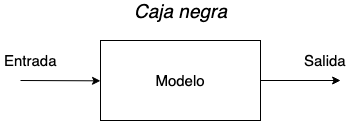
\includegraphics[scale=0.6]{mem/images/cap-1/1-1.png}
    \caption{Esquema general de un modelo computacional de caja negra}
    \label{fig:my_label}
\end{figure}

Este esquema que hemos definido es muy conveniente para establecer un criterio de clasificación de problemas, en función de que partes del sistema son conocidas y cuales no. A partir de esto podemos diferenciar en tres tipos de problemas:

\subsubsection{Optimización}
Los problemas de optimización son aquellos en los que se conoce el modelo, además de la salida que se espera, o al menos una descripción de la misma, y en función de ello, se debe calcular cuales son los valores de entrada que proporcionan dicha salida. \\

Existen multitud de problemas que se clasifican en esta categoría, aunque quizás uno de los más clásicos es el problema de viajante de comercio (\textbf{TSP}). Este problema consiste en encontrar la secuencia de rutas de coste mínimo dado un grafo de ciudades y sus interconexiones, de tal forma que cada una de las ciudades sea visitada solo una vez.\\

Como vemos, en este problema está especificada cual es la salida esperada, además del modelo de computación, sin embargo, lo que desconocemos es cual será la entrada, es decir, la combinación de rutas que minimizará el coste y que satisface las restricciones.

\subsubsection{Modelización}

En los problemas de modelización, se conocen las entradas y sus correspondientes salidas, pero se desconoce cual es el modelo de computación que debe usarse para procesarlas. \\


Este es el tipo de problemas que se abordan en áreas como el \textbf{Machine Learning}, pues en ellos se suele tener un conjunto de datos en los que existe una correspondecia entre las entradas y su resultado esperado. El problema está en crear un modelo que sea capaz de \textit{aprender} a partir de dichos datos y por tanto, sea capaz de generalizar y extraer características de datos que no haya procesado previamente.

\subsubsection{Simulación}

Este es el tipo de problemas más lineales, pues en ellos se conoce cuales serán las entradas y el modelo de computación, pero se desconoce cual será la salida. \\

Existen multitud de ejemplos de problemas de simulación, como por ejemplo; simulación de fluidos, o simulación meteorológica. Este tipo de problemas tienen una gran utilidad, pues nos permiten predecir una realidad futura, lo cual es crucial en múltiples ámbitos. \\

%------

\subsection{Clasificación en función de la complejidad (Clases P y NP)}

Otra clasificación posible que se puede hacer de los problemas es en función de la \textit{complejidad} que entraña resolverlos. De esta forma una clasificación básica en este sentido pueden ser los problemas \textit{fáciles} y \textit{difíciles} de resolver.\\

Esta definición puede resultar ambigua, puesto que existen múltiples algoritmos que pueden resolver un problema. Es por ello, que para medir la complejidad de un problema, elegimos el algoritmo que lo resuelve en menor tiempo. Con \\textbf{tiempo de ejecución} realmente no nos referimos a una magnitud física, sino al número de pasos elementales u operaciones que lleva finalizarlo. \\

Atendiendo a esta clasificación, nos encontramos 3 clases de problemas:

\begin{itemize}
    \item \textbf{Clase $\mathcal{P}$}: Los problemas que pertenecen a la clase $\mathcal{P}$, son aquellos en los que existe un algoritmo que pueda resolverlos en tiempo polinomial. Es decir que la función que expresa la complejidad temporal de resolución del algoritmo, es un polinomio.
    \item \textbf{Clase $\mathcal{NP}$}: Para los problemas que están en $\mathcal{NP}$ no existe un algoritmo que pueda resolverlos en tiempo polinomial, sin embargo, se puede evaluar si una solución es válida para el problema en tiempo polinomial. Por ejemplo, el TSP o el VRP son problemas que pertenecen a esta clase.
    \item \textbf{Clase $\mathcal{NP}-Completo$}: Este es un subconjunto de problemas de $\mathcal{NP}$, que se corresponden con los problemas mas difíciles de resolver. Se considera que un problema es $\mathcal{NP}$-Completo cuando está en $\mathcal{NP}$ y además, \textbf{todos} los problemas de $\mathcal{NP}$ se pueden transformar a dicho problema mediante una \textbf{reducción polinomial}. Encontrar un problema que pertenenciera a esta clase fue una tarea compleja hasta el desarrollo del \textbf{Teorema de Cook}.
\end{itemize}

Uno de los problemas que más trae de cabeza a la comunidad científica, considerado como una de las grandes incógnitas de la matemática moderna es el problema ¿$\mathcal{P} = \mathcal{NP}$? Este problema trata de discernir si verdaderamente existen problemas que están en $\mathcal{NP}$ porque tienen una naturaleza diferente a los que están en $\mathcal{P}$, o es porque aún no hemos encontrado un algoritmo lo sufiecientemente bueno para resolverlo en un tiempo razonable.

%---------------------------------------------------------------------------------
\section{Computación evolutiva}
\label{1:sec:2}

Como podemos ver, existe una gran cantidad de problemas que no poseen un algoritmo exacto que los pueda resolver en un tiempo razonable. Es por ello, que se necesita buscar alternativas que nos permitan llevar a cabo la resolución de dichos problemas, aunque muchas veces se deba hacer de manera aproximada. \\

La computación evolutiva es una técnica que nos permite encontrar las soluciones a dichos problemas complejos, inspirándose en el proceso evolutivo natural para lograr los resultados. El proceso natural de evolución tiene mucho potencial a la hora de construir buenas soluciones a los problemas, principalmente porque se potencia el mecanismo de "\textit{prueba y error}". \\

En el proceso evolutivo natural, contamos con un ambiente en el que se encuentran una serie de recursos, por los cuales tienen que competir los individuos que se encuentren en él. Además de tratar de obtener la mayor parte de los recursos disponibles, los individuos tratarán de reproducirse entre sí. De esta forma, en las sucesivas generaciones de individuos, solo los más daptados habrán conseguido sobrevivir y transmitir sus características físicas a su descendencia, a través del material genético. \\

Mediante un algoritmo evolutivo, se trata de simular este mismo procedimiento. Para ello, consideramos que el ambiente que contiene los recursos por los que los individuos deben competir es el problema que queremos solucionar, y las posibles soluciones del problema son los individuos. Para simular el grado de adaptación al ambiente que deben tener estos individuos se utilizará una función que medirá cual buena es la solución que se está evaluando. Al igual que ocurre en un ambiente real, estos individuos deberán reproducirse entre sí, transmitiendo su material \textit{genético} a la descendencia. \\

%---------------------------------------------------------------------------------
\section{Algoritmos evolutivos}
\label{1:sec:3}

Siguiendo la idea básica que se quiere perseguir con los algoritmos evolutivos, podemos construir un esquema para determinar cuales serán las distintas fases que tendrán este tipo de algoritmos:

\begin{algorithm}[H]
 INICIALIZAR la población con $n$ individuos aleatorios;\\
 EVALUACIÓN de la población mediante la función de fitness;
 
 \While{CONDICIÓN DE PARADA no sea satisfecha}{
  SELECCIÓN de padres; \\
  RECOMBINACIÓN de pares de padres; \\
  MUTACIÓN de la descendencia; \\
  EVALUCACIÓN de la descendencia; \\
  SELECCIÓN de supervivientes para la siguiente generacón;
 }
 \caption{Esquema básico de un algoritmo evolutivo}
\end{algorithm}

En este esquema podemos ver las diferentes fases de las que se compone un algoritmo evolutivo. En primer lugar, se deberá inicializar una población con individuos generados aleatoriamente, que se corresponderán con las posibles soluciones que puede tener nuestro problema, a continuación estás soluciones deberán ser evaluadas mediante la función de fitness, determinando así su grado de adaptación al medio. \\

Seguidamente, se entrará en el bucle principal del algoritmo, el cual continuará ejecutándose mientras que una determinada condición de parada no haya sido satisfecha. Dentro de este bucle, se aplicarán los operadores principales sobre la población generada; en primer lugar, se seleccionarán los padres que se reproducirán en la siguiente generación, a los cuales se les aplicará un operador de cruce para generar una descendencia. Esta descendencia, sufrirá de manera aleatoria una mutación que afectará a su material genético, y después de ello, se evaluará de nuevo respecto a la función de fitness. Seguidamente, se deberán seleccionar que individuos son los que permanecerán en la siguiente generación, repitiendo de nuevo el bucle. \\

Podemos afirmar que este es un procedimiento estocástico, puesto que en él están involucrados numerosos componentes aleatorios. Esta aleatoriedad es el motor principal de las dos fuerzas que garantizan la eficacia de este tipo de algoritmos:

\begin{itemize}
    \item \textbf{Variación}: Los operadores de variación (recombinación y mutación), generan la suficiente diversidad como para explorar una gran parte del espacio de soluciones.
    \item \textbf{Intensificación}: Los operadores de selección tanto de padres como de descendencia, son los responsables de que se exploren las mejores soluciones garantizando que su material genético perviva en sucesivas generaciones.
\end{itemize}

Para cada una de las fases de las que se compone un algoritmo evolutivo, existen numerosos métodos que se pueden aplicar. Los cuales dependen enormemente de la codificación que se le esté aplicando a los individuos, además del problema concreto que se esté tratando de resolver.